\pdfoutput=1  % arXiv: build with pdfLaTeX (PDF figures)
\documentclass[runningheads]{llncs}

% ---------------------------------------------------------------
% A General Variable Neighborhood Search for a logistic transport
% network design problem with nonlinear edge costs and transshipment
% capacity constraints.
%
% arXiv version.  Identical in content to the version submitted to a
% Springer LNCS conference; the only additions are \pdfoutput=1 and the
% hyperref PDF metadata.
% Build:  pdflatex logistics_gvns  (twice, no BibTeX -- the
% bibliography is a manual thebibliography environment).
% ---------------------------------------------------------------

\usepackage[utf8]{inputenc}
\usepackage[T1]{fontenc}
\usepackage{lmodern}
\usepackage{amsmath,amssymb}
\usepackage{mathtools}
\usepackage{graphicx}
\usepackage{booktabs}
\usepackage{array}
\usepackage{caption}
\usepackage{subcaption}
\usepackage{multirow}
\usepackage{float}
\usepackage{enumitem}
\usepackage[hidelinks]{hyperref}
\usepackage{xcolor}

% PDF metadata (arXiv version)
\hypersetup{
  pdftitle={A General Variable Neighborhood Search for Logistic Network Flow
            Design with Nonlinear Edge Costs and Transshipment Capacities},
  pdfauthor={Varvara Kovaleva, Alexander Ponomarenko},
  pdfsubject={Multi-commodity network flow design; variable neighborhood search},
  pdfkeywords={multi-commodity flow, network design, variable neighborhood
               search, metaheuristics, mixed integer programming, logistics}
}

\captionsetup{font=small,labelfont=bf}


\usepackage{placeins}  % \FloatBarrier -- keep floats out of the reference list
% Formal algorithm typesetting
\usepackage[ruled,vlined,linesnumbered]{algorithm2e}
\SetKwProg{Fn}{Function}{:}{}
\SetKwFunction{PN}{ProcessNeighborhood}
\SetKwFunction{GenPaths}{GenPaths}
\SetKwFunction{SolveMILP}{SolveMILP}
\SetKwFunction{RoundedLP}{RoundedLP}

% Convenient operators
\DeclareMathOperator*{\argmin}{arg\,min}
\newcommand{\E}{E}
\newcommand{\Vv}{V}
\newcommand{\Real}{\mathbb{R}}
\newcommand{\Int}{\mathbb{Z}}

% llncs sets \flushbottom, so short pages are filled by stretching whatever
% vertical glue they contain -- which on text pages means the \paragraph skips,
% inflating them from 12pt to nearly 30pt.  \raggedbottom keeps those skips at
% their natural size and leaves the slack at the foot of the page instead.
\raggedbottom

\begin{document}

\title{A General Variable Neighborhood Search for Logistic Network
Flow Design with Nonlinear Edge Costs and Transshipment Capacities}
\titlerunning{GVNS for Logistic Network Flow Design}


\author{Varvara Kovaleva \inst{1} \and Alexander Ponomarenko\inst{2} }
\authorrunning{V. Kovaleva and A. Ponomarenko}
\institute{
HSE University, Nizhny Novgorod, Russia\\
\email{varvara\_kovaleva03@mail.ru}
\and
Laboratory of Algorithms and Technologies for Network Analysis, HSE University, Nizhny Novgorod, Russia\\
\email{aponomarenko@hse.ru}\\
}

\maketitle

\begin{abstract}
We study how to route multiple commodities through a logistic transport network
so as to minimise the joint cost of vehicle movements and of transshipment
(reload) operations at intermediate storages. The problem combines
two features common in practice but rarely treated together: edge costs that are
\emph{nonlinear} in the transported volume, because freight is carried by
vehicles of fixed capacity, and \emph{hard upper bounds} on the volume that can
be reloaded at each node. We formulate it as a mixed integer linear program in
both an arc-based and a path-based form, derive its linear relaxation, and
propose a solver based on General Variable Neighborhood Search (GVNS). The method
works in the path space and relies on three problem-specific neighborhoods that
generate candidate paths by (i)~shortest paths under a reload-aware metric,
(ii)~edges carrying partially loaded vehicles, and (iii)~detours around congested
storages. We evaluate it on our open benchmark~\cite{benchmark}: realistic
logistic networks calibrated on real road graphs of nine European countries, five
U.S.\ states and the European part of Russia. On 35 synthetic and 15
real-geometry instances with up to 150 storages, GVNS returns solutions within
about one percent of the best dual bound on small networks---a branch-and-bound
lower bound substantially tighter than the LP relaxation---is stable across
random seeds, and for a comparable wall-clock budget is up to $55\%$ better than
a time-limited exact solver on the medium instances.

\keywords{multi-commodity flow \and network design \and variable neighborhood
search \and metaheuristics \and mixed integer programming \and logistics}
\end{abstract}

\section{Introduction}

Organising commodity flows between distribution centres is a central problem of
logistic networks, and the scale of modern warehousing keeps demand for efficient
planning algorithms high. Two features make realistic instances hard. First, the
cost of using a road is \emph{nonlinear} in the volume carried: goods travel in
vehicles of fixed capacity, so the billed quantity is the integer \emph{number of
vehicles}, obtained by rounding the volume up to that capacity. Second, every
storage has a limited \emph{transshipment capacity}---an upper bound on the volume
that may be unloaded, stored and reloaded there. Together they turn an otherwise
classical multi-commodity flow problem into a mixed integer program with node
capacities and a step-wise vehicle cost term.

\paragraph{Related work.} The problem belongs to the family of capacitated
multicommodity network design (MCND)~\cite{gendron1999,crainic2000}, which is
NP-hard. Exact approaches solve path-based formulations by column generation and
branch-and-price~\cite{barnhart1998}; at practical scale heuristics dominate,
notably cycle-based neighbourhoods inside tabu search~\cite{ghamlouche2003},
local branching~\cite{rodriguez2010} and matheuristics that call a MILP solver on
restricted subproblems~\cite{hewitt2010}. Metaheuristics for multi-commodity flow
more broadly are surveyed in~\cite{crainic2021}. Cost functions of the kind
studied here appear as \emph{step} or discrete costs: Gabrel et
al.~\cite{gabrel1999} give an exact Benders-type procedure for general step
costs, and Croxton et al.~\cite{croxton2003} compare MILP models of nonconvex
piecewise-linear costs. Capacity on the \emph{node} side is instead typical of
hub location, where hub throughput is bounded~\cite{alumur2008}. Variable
Neighborhood Search~\cite{mladenovic1997,hansen2019,hansen2017} has proven
effective across a broad range of optimisation problems: Masri et
al.~\cite{masri2015} applied a multi-start VNS to the single-path
multi-commodity flow problem, General VNS performs well on capacitated vehicle
routing and other flow-constrained logistic problems~\cite{amous2017}, and
problem-specific heuristics do well on real-life logistic routing, such as the
truck-and-trailer routing problem with time windows and split
deliveries~\cite{batsyn2014ttrp,batsyn2015heuristic}.

No third-party solver targets the variant studied here: published MCND codes
charge a \emph{fixed} cost per open arc rather than a per-vehicle step cost, and
none of them bounds the volume transshipped at a node, so a head-to-head comparison
would be between different problems. Nor are there published results to compare
with, since the instance corpus we published earlier~\cite{benchmark,benchmark-data}
supplies networks and demands but no solutions. The evaluation below is therefore
against bounds and general-purpose solvers on the identical model, and it
establishes the first reference values on that corpus.

\paragraph{Contributions.} We formalise the problem and give equivalent arc-based
and path-based MILP models with their linear relaxation
(Section~\ref{sec:model}); we design a GVNS that searches the space of commodity
paths through three problem-specific neighborhoods, which exploit reload costs,
partial vehicle loads and storage congestion (Section~\ref{sec:gvns}); and we
report a computational study on that corpus
(Section~\ref{sec:data}) comparing GVNS against the LP relaxation, its rounded
version, and the dual bounds and incumbents of an exact solver
(Section~\ref{sec:experiments}), together with a component analysis that isolates
the contribution of each neighborhood and of the VND itself.

\section{Problem statement and model}
\label{sec:model}

\subsection{Problem description}
Consider a directed graph $G=(\Vv,\E)$ whose nodes are storages and whose edges
are roads. Each storage $v\in \Vv$ has a per-unit reload cost $f_v\in\Real_+$ and
a hard \emph{transshipment capacity} $W_v\in\Real_+$, the largest volume that may
be unloaded, stored and reloaded there; each edge $e\in \E$ has a per-vehicle
traversal cost $c_e\in\Real_+$. Freight moves in vehicles of capacity
$C\in\Real_+$, so what an edge actually costs is set by the \emph{integer} number
of vehicles it carries. We are given a set $K$ of transportation requests
(commodities); request $k\in K$ must ship a demand $d_k\in\Real_+$ from an origin
$s_k\in \Vv$ to a destination $t_k\in \Vv$.

The problem is to route all requests so as to minimise the total vehicle movement
cost plus the total transit reload cost, subject to demand satisfaction, edge
vehicle capacities and node transshipment capacities. It is thus a capacitated
multi-commodity network design problem with step edge costs and node
transshipment capacities, and it admits two equivalent formulations, arc-based
and path-based, given next. Capacities and costs are treated as constants; on
real networks they vary with the time of day, a point we return to in
Section~\ref{sec:concl}.

\subsection{Mathematical model}
\textbf{Decision variables.} \emph{Arc-based:} let $x^k_e\in\Real_+$ be the flow
of commodity $k\in K$ on edge $e\in \E$ and $y_e\in\Int_+$ the number of vehicles
traversing $e$; the model has $|K|\cdot|\E|+|\E|$ variables. \emph{Path-based:}
let $\Pi_k$ be the set of all paths from $s_k$ to $t_k$, let $x^k_p\in\Real_+$ be
the flow of commodity $k$ on path $p\in\Pi_k$, and $y_e\in\Int_+$ as above; the
model has $\sum_{k\in K}|\Pi_k|+|\E|$ variables.

\smallskip\noindent\textbf{Objective.} With $\delta^-(v)\subseteq \E$ and
$\delta^+(v)\subseteq \E$ the sets of edges entering and leaving $v$, minimise
vehicle movement cost (first term) plus transit reload cost (second term).

\noindent\emph{Arc-based:}
\begin{equation}
\min\;\Bigg(\sum_{e\in \E} c_e\,y_e
 \;+\!\!\sum_{k\in K}\;\sum_{\substack{v\in \Vv\\ v\neq s_k,\,v\neq t_k}}
 \sum_{e\in\delta^-(v)} f_v\,x^k_e\Bigg).
\label{eq:obj-arc}
\end{equation}

\noindent\emph{Path-based:}
\begin{equation}
\min\;\Bigg(\sum_{e\in \E} c_e\,y_e
 \;+\!\!\sum_{k\in K}\;\sum_{p\in\Pi_k}\;
 \sum_{\substack{v\in p\\ v\neq s_k,\,v\neq t_k}} f_v\,x^k_p\Bigg).
\label{eq:obj-path}
\end{equation}

\smallskip\noindent\textbf{Constraints.} \emph{(1) Demand satisfaction.}
\begin{align}
\text{arc:}\quad
&\sum_{e\in\delta^+(v)} x^k_e-\sum_{e\in\delta^-(v)} x^k_e=
 \begin{cases} d_k, & v=s_k\\ -d_k, & v=t_k\\ 0, & \text{otherwise}\end{cases}
 \quad \forall k\in K,\ \forall v\in \Vv;
 \label{eq:demand-arc}\\[2pt]
\text{path:}\quad
&\sum_{p\in\Pi_k} x^k_p=d_k, \qquad \forall k\in K.
\label{eq:demand-path}
\end{align}

\noindent\emph{(2) Vehicle capacity on edges.} Enough vehicles must run on each
edge to carry the total flow:
\begin{align}
\text{arc:}\quad &\sum_{k\in K} x^k_e\le C\,y_e, \qquad \forall e\in \E;
\label{eq:cap-arc}\\
\text{path:}\quad &\sum_{k\in K}\sum_{p\in\Pi_k:\,e\in p} x^k_p\le C\,y_e,
\qquad \forall e\in \E.
\label{eq:cap-path}
\end{align}

\noindent\emph{(3) Storage transshipment capacity.}
\begin{align}
\text{arc:}\quad
&\sum_{\substack{k\in K\\ v\neq s_k,\,v\neq t_k}}\sum_{e\in\delta^-(v)} x^k_e
 \le W_v, \qquad \forall v\in \Vv;
\label{eq:node-arc}\\
\text{path:}\quad
&\sum_{\substack{k\in K\\ v\neq s_k,\,v\neq t_k}}\sum_{p\in\Pi_k}
 \sum_{v\in p} x^k_p \le W_v, \qquad \forall v\in \Vv.
\label{eq:node-path}
\end{align}

\subsection{Complexity and linear relaxation}
\label{sec:relax}
The objective and all constraints are linear and the variables are mixed---the
vehicle counts $y_e$ are integer while the flows $x^k_e$ (or $x^k_p$) are
continuous---so the problem is a \emph{mixed integer linear program} (MILP), an
NP-hard class for which no polynomial-time exact algorithm is known in general.

A standard way to bound the optimum is the LP relaxation: dropping the
integrality of $y_e$ turns the MILP into a linear program solvable in
polynomial time, and its optimum is a lower bound (for minimisation). Once
$y_e$ is continuous, the capacity constraints \eqref{eq:cap-arc}--%
\eqref{eq:cap-path} hold with equality at optimum, so $y_e$ can be eliminated:
\begin{equation}
y_e=\frac1C\sum_{k\in K} x^k_e \quad(\text{arc}), \qquad
y_e=\frac1C\sum_{k\in K}\sum_{p\in\Pi_k:\,e\in p} x^k_p \quad(\text{path}).
\label{eq:ye-relax}
\end{equation}
Substituting \eqref{eq:ye-relax} into the objective yields a relaxed problem
in the flow variables only. In the path-based form,
\begin{equation}
\min\;\sum_{k\in K}\sum_{p\in\Pi_k} x^k_p
\Bigg(\frac1C\sum_{e\in p} c_e+\sum_{\substack{v\in p\\ v\neq s_k,\,v\neq t_k}}
f_v\Bigg),
\label{eq:relax-path}
\end{equation}
which makes explicit that an optimal relaxed solution prefers paths with low
travel cost and few transit nodes.

\section{The GVNS solution approach}
\label{sec:gvns}

\subsection{General Variable Neighborhood Search}
VNS~\cite{hansen2019,hansen2017} is a metaheuristic whose core idea is the
systematic change of neighborhood structures while exploring the solution space.
Given a problem $\min\{f(x):x\in X\}$ and a family of neighborhoods
$N_k(x),\ k=1,\dots,k_{\max}$, the classical scheme alternates three steps: a
\emph{shake} (a random move in $N_k$ to escape local optima), a \emph{local
search}, and a \emph{neighborhood change} (on improvement, accept the move and
reset $k\!\gets\!1$; otherwise advance to $k\!+\!1$). When the local search is
itself a Variable Neighborhood Descent (VND)---a deterministic sweep through the
neighborhoods ordered from intensification to diversification---the method is
called General VNS (GVNS), which often outperforms single-neighborhood
heuristics~\cite{karakostas2019,mjirda2014}. Our instantiation searches the space
of commodity paths; its concrete form is Algorithm~\ref{alg:gvns}, built on the
neighborhood-processing primitive of Algorithm~\ref{alg:pn}.

\subsection{Preprocessing and initial solution}
Transport networks are typically sparse directed graphs in which not every
pair of storages is joined by a direct road, and not every transit node needs
a reload. Working on the raw graph both shrinks the feasible region (through
node capacities) and may even render the instance infeasible if no path exists
between an origin and a destination.

To avoid this, the graph is \emph{completed}: for every pair of storages
$v,u$ we add (or update) an edge whose cost equals that of the shortest path
from $v$ to $u$ in $G$. Each edge of the resulting complete graph thus
represents the cheapest stop-free route between its endpoints, and $c_{vu}$
denotes its per-vehicle cost. From here on $G=(\Vv,\E)$ denotes this completed
graph, so every later formula ranges over all ordered pairs of storages. This guarantees
the existence of a feasible solution, because flow routed on the direct
origin--destination edge does not pass through any transit node and hence
violates no node-capacity constraint. From the relaxed objective
\eqref{eq:relax-path} it follows that the cheapest, transit-free direct edges
are exactly the ones a good solution prefers. We therefore take as the initial
solution the relaxed LP solution that sends each commodity entirely along its
direct origin--destination edge, with vehicle counts rounded up:
\begin{equation}
y_e=\Big\lceil \tfrac1C\sum_{k\in K} x^k_e\Big\rceil, \qquad \forall e\in \E.
\label{eq:init}
\end{equation}

\subsection{Neighborhoods}
Since the vehicle counts $y_e$ are determined directly from the flows via
\eqref{eq:init}, the neighborhoods vary the flows. Predicting feasible
per-edge flows is hard because edges are shared by many commodities and
adjacent flows are strongly coupled, so the whole network must be considered
at once. A single path, by contrast, describes the routing of just one
commodity, and adding a new path to an already feasible solution never worsens
it. The neighborhoods therefore \emph{build and modify the set of candidate
paths for each commodity}: for every commodity a set of new paths is generated
and added to the model, a MILP solver is run for a limited time to
redistribute flow, and---if the objective improves---all new paths carrying
nonzero flow are kept. Three neighborhoods define how the new paths are
generated.

\paragraph{N1 -- Shortest paths (reload-aware).}
Classical shortest-path search ignores reload costs. We instead build an
auxiliary complete graph $G'$ whose edge weights measure the per-unit cost of
moving one unit of commodity, including reloads at the endpoints:
\begin{equation}
c'_{vu}=f_v+f_u+\frac{c_{vu}}{C}, \qquad \forall (v,u)\in \E .
\end{equation}
Before GVNS starts, a pool of shortest paths under $c'$ is precomputed for each
commodity; new paths are then drawn from it, either at random or preferring
low-cost paths. During VND all combinations of the two parameters---the number of
new paths per commodity and the selection strategy---are swept (one to three
paths, both strategies); in Shake, five random paths are always added, which helps
escape local optima.

\paragraph{N2 -- Partially loaded edges.}
A partially loaded vehicle has spare room: routing extra flow over such an edge
can free another vehicle and reduce the vehicle count. For every edge we
compute, for every $e\in \E$, the residual load $load_e=\big(\sum_{k\in
K}\sum_{p\in\Pi_k:\,e\in p} x^k_p\big) \bmod C$, and build a graph $G''$ that
favours edges with free capacity. Fully loaded
edges ($load_e=0$) are least attractive, since new flow would require an extra
vehicle, and keep their weight from $G'$. The remaining edges receive
\begin{equation}
c''_{vu}=f_v+f_u+\frac{load_{vu}}{C}\Big(\frac{c_{vu}}{C}\Big)^{\!\alpha},
\qquad \alpha\le 1,
\end{equation}
so that smaller residual load (more free room) lowers the weight and raises
priority; $\alpha$ tunes how strongly travel cost influences the weight, and
shortest-path search on $G''$ then tends to build paths through partially loaded
vehicles. The number of new paths is set dynamically: a counter of fully loaded
paths and an accumulator of total free room stop generation once a threshold is
reached (in VND, at most two fully loaded paths or free room above one vehicle
capacity; in Shake, three paths and $5C$).

\paragraph{N3 -- Detours around congested storages.}
Storages whose transshipment volume is at or near their capacity are
bottlenecks, and routing around them is desirable. For the current solution we
compute, for every $v\in \Vv$, a congestion ratio
$overload_v=\frac1{W_v}\sum_{k\in K,\,v\neq s_k,t_k}\sum_{p\in\Pi_k}\sum_{v\in p}
x^k_p$. Storages are sorted by decreasing $overload_v$ and the single most
congested one is deleted from $G'$ (except where it is the commodity's own origin
or destination); a shortest path is then recomputed, yielding detours that bypass
the busiest node and shift flow to less loaded ones. One new path per commodity is
generated in VND and three in Shake. The natural generalisation---removing a whole
prefix of $|\Vv|/5$--$|\Vv|/4$ congested storages---was also tried: over all $50$
instances and ten seeds it is indistinguishable from the single-node rule ($44$ of
$50$ instances within across-seed noise) yet forfeits $N_3$'s benefit on the
capacity-tight networks, so we keep the surgical version.

\begin{algorithm}[t]
\DontPrintSemicolon
\Fn{\PN{$P,\ x,\ z,\ N,\ \mathit{div},\ \tau$}}{
  \tcp{path pool $P$, flows $x$, objective $z=f(x)$; all updated in place}
  $Q \gets \bigcup_{k \in K}{}$ \GenPaths{$N,\ k,\ \mathit{div}$}\tcp*{candidates; $N$ selects the rule}
  \lIf{$Q = \emptyset$}{\Return \textbf{false}}
  $(x',\ z') \gets{}$ \SolveMILP{$P \cup Q,\ x,\ \tau$}\tcp*{redistribute; warm start $x$, limit $\tau$}
  \lIf{$z' \ge z$}{discard $Q$; \Return \textbf{false}}
  $P \gets P \cup \{\, p \in Q : x'_p > 0 \,\}$;\ \ $x \gets x'$;\ \ $z \gets z'$\;
  prune from $P$ every path carrying zero flow\tcp*{keep the model bounded}
  \Return \textbf{true}
}
\caption{\texttt{ProcessNeighborhood}: enlarge the path pool, re-optimise the
flows by MILP, and keep the move iff it improves the objective.}
\label{alg:pn}
\end{algorithm}

\begin{algorithm}[t]
\DontPrintSemicolon
\SetKwInOut{Input}{Input}\SetKwInOut{Output}{Output}
\Input{graph $G=(\Vv,\E)$, commodities $K$, vehicle capacity $C$, time limit $t_{\max}$}
\Output{path pool $P$ with commodity flows $x$}
build the reload-aware complete graph $G'$; precompute a shortest-path pool per commodity\;
$P \gets \{\,(s_k,t_k) : k \in K\,\}$;\ \ $(x,z) \gets{}$ \RoundedLP{$P$}\tcp*{initial solution, Eq.~\eqref{eq:init}}
$k \gets 1$\;
\While{$k \le 3$ \textbf{\emph{and}} $\mathrm{CpuTime} < t_{\max}$}{
  \PN{$P,\ x,\ z,\ N_k,\ \textbf{true},\ \tau_{\mathrm{shk}}$}\tcp*{shake: diversified, larger budget}
  $z_0 \gets z$\;
  \Repeat{$\neg\,\mathit{imp}$ \textbf{\emph{or}} $\mathrm{CpuTime} \ge t_{\max}$}{
    $\mathit{imp} \gets{}$ \PN{$P,\ x,\ z,\ N_1,\ \textbf{false},\ \tau_{\mathrm{vnd}}$}\;
    \lIf{$\neg\,\mathit{imp}$}{$\mathit{imp} \gets{}$ \PN{$P,\ x,\ z,\ N_2,\ \textbf{false},\ \tau_{\mathrm{vnd}}$}}
    \lIf{$\neg\,\mathit{imp}$}{$\mathit{imp} \gets{}$ \PN{$P,\ x,\ z,\ N_3,\ \textbf{false},\ \tau_{\mathrm{vnd}}$}}
  }
  \leIf{$z < z_0$}{$k \gets 1$}{$k \gets k+1$}\tcp*{neighborhood change}
}
\Return $(P,\ x)$
\caption{\texttt{GVNS} for logistic network flow design.}
\label{alg:gvns}
\end{algorithm}

\subsection{Overall algorithm}
Algorithm~\ref{alg:pn} is the primitive shared by the three neighborhoods. Only
the generation step \GenPaths\ differs between $N_1$, $N_2$ and $N_3$.
Algorithm~\ref{alg:gvns} embeds it in the GVNS template: starting from the
rounded-LP solution of Eq.~\eqref{eq:init}, each round shakes with the current
neighborhood---diversified parameters and a larger MILP budget
$\tau_{\mathrm{shk}}$---and then runs the VND sweep $N_1\!\to\!N_2\!\to\!N_3$ with
a smaller budget $\tau_{\mathrm{vnd}}$, since VND explores a narrower region. The
neighborhood index resets on improvement and advances otherwise; a global limit
$t_{\max}$ bounds the run, and the search stops once a full sweep brings no
improvement.


\section{Benchmark instances}
\label{sec:data}

We evaluate GVNS on our open benchmark~\cite{benchmark,benchmark-data}, published
as a Zenodo dataset (CC-BY-4.0); we summarise only what the study needs and refer
to~\cite{benchmark} for the generator. The corpus targets upper-level road networks
connecting regional sorting centres, calibrated on OpenStreetMap~\cite{osm} data
for nine European countries, five large U.S.\ states and the European part of
Russia. It reproduces the structural statistics of real regional transport
systems---Zipf city sizes~\cite{gabaix1999}, a spatial-network budget
topology~\cite{gastner2006}, centrality-driven transshipment
capacities~\cite{barthelemy2011,kirkley2018} and a doubly constrained gravity
demand model~\cite{wilson1967}---yielding \emph{near-planar, large-diameter} graphs
(mean degree about $3.575$), the opposite of small-world networks.
The corpus comprises $35$ synthetic instances ($10$ with $10$ storages, $7$ each
with $20$ and $30$, $5$ with $50$, and $3$ each with $100$ and $150$) and $15$
real-geometry instances built on the calibration road graphs ($11$--$90$
storages); we use all $50$, each exactly reproducible from its published seed and
parameters.

\section{Computational experiments}
\label{sec:experiments}

\subsection{Setup, baselines and metric}
All experiments were run on the HPC cluster ``cHARISMa''~\cite{charisma} (nodes
with two AMD~EPYC CPUs, 44~cores and $\ge$720\,GB RAM, Rocky~Linux~9), each job
pinned to eight cores. The exact models were solved with HiGHS~1.14.0~\cite{highs}
and, as an independent cross-check of the lower bounds, with
SCIP~10.0.2~\cite{scip}; HiGHS is also the metaheuristic's in-loop redistribution
solver. GVNS is stochastic (random path
choices in the shake step), so every instance was solved with ten independent
random seeds and we report the best objective together with its across-seed
mean and standard deviation; the component studies of
Section~\ref{sec:ablation}, which compare variants rather than establish the
headline numbers, use five seeds each. Unless stated otherwise the exact solves were run
to a target MIP gap of zero (i.e.\ to optimality where possible) under
a size-dependent wall-clock budget (30~min for $|V|=10$, growing to 4~h for
$|V|=150$); GVNS is run with a time limit of twice the number of storages, in
minutes. The two budgets are comparable---at $|V|=50$, for example, GVNS is
allowed $100$~min against the exact solver's $2$~h, and at $|V|=10$ it is
$20$~min against $30$~min.

The main settings are collected in Table~\ref{tab:params}. The arc-based MIP
grows steeply with $|V|$---from about $6\,000$ variables at $|V|=10$ ($|E|=90$,
$|K|=67$) to $3.7\times10^{8}$ at $|V|=150$ ($|E|=22\,350$, $|K|=16\,762$)---which
is why it becomes intractable well before that size, while GVNS, working in the
much smaller path space, remains applicable throughout.

\begin{table}[t]
\centering
\caption{GVNS and exact-solver settings. Values that differ between the VND and
the Shake step are given as VND\,/\,Shake.}
\label{tab:params}
\small
\setlength{\tabcolsep}{3pt}
\begin{tabular}{llll}
\toprule
Setting & Value & Setting & Value\\
\midrule
Neighborhoods $k_{\max}$ & $3$
  & $N_2$ exponent $\alpha$ & $0.5$\\
GVNS limit $t_{\max}$ & $2|V|$\,min
  & $N_2$ free-room stop & $1C$\,/\,$5C$\\
Random seeds & $10$\,/\,$5$
  & $N_3$ storages removed & $1$ (worst)\\
Vehicle capacity $C$ & $50$
  & $N_1$ path pool & $20$\\
$N_1$ paths/commodity & $1$--$3$\,/\,$5$
  & $N_3$ paths/commodity & $1$\,/\,$3$\\
Init.\ MILP limit & $300$\,s
  & Exact gap target & $0$\\
Redistrib.\ MILP gap & $1\%$
  & Exact budget & $30$\,min--$4$\,h\\
$\tau_{\mathrm{shk}}$ ($N_1$\,/\,rest) & $10{+}|V|$\,/\,$100{+}2|V|$\,s
  & $\tau_{\mathrm{vnd}}$ ($N_1$\,/\,rest) & $25$\,/\,$70$\,s\\
\bottomrule
\end{tabular}
\end{table}

Lacking known optima, we compare GVNS against four references. The \emph{LP
relaxation} (Section~\ref{sec:relax}) is a lower bound; on the completed graph it
is attained by routing every commodity along its direct edge
(Section~\ref{sec:gvns}), so it is available in closed form at every size, but
ignoring vehicle integrality makes it loose. The \emph{rounded LP}---the relaxed
solution with $y_e$ rounded up---is the GVNS starting solution and a valid upper
bound. The \emph{MIP dual bound} is the global lower bound of the exact solver's
search tree, i.e.\ the LP relaxation strengthened by branching and cutting planes,
which rises towards the optimum as the tree is explored; it is a valid lower bound
($\underline{z}\le z^{\ast}$) that, unlike the root relaxation, is typically tight
(within a few percent of the incumbent), and it is our key reference because it
bounds the true optimum even when optimality is not proved. Finally, the \emph{MIP
incumbent} is the best feasible solution the exact solver returns within a budget
comparable to the GVNS run time.

Because the true optimum is generally not available, the primary quality
measure we report is the \emph{optimality gap of GVNS to the best valid lower
bound},
\[
  gap_{\mathrm{LB}}=\frac{Result_{\text{GVNS}}-\underline{z}}{\underline{z}},
  \qquad
  \underline{z}=\text{best MIP dual bound},
\]
which upper-bounds the true optimality gap of GVNS. We additionally report the
ratio of each reference objective to that of GVNS
($Ratio_{\text{method}}=Result_{\text{method}}/Result_{\text{GVNS}}$), so values
below~$1$ are better than GVNS and above~$1$ are worse.

\paragraph{On the hardness of the exact model.} The arc-based MILP is hard even
at the smallest sizes: with the vehicle-count integrality it is a large mixed
integer program ($\sim\!6000$ variables already at $|V|=10$), and \emph{no}
instance was solved to \emph{proven} optimality within the budgets above by either
solver. The branch-and-bound dual bound, however, is tight and well above the LP
relaxation, which makes it the right yardstick for GVNS. The two solvers behave
very differently on this model: up to $|V|=42$ their dual bounds agree to within
$0.6\%$ (mean $0.18\%$), mutually cross-validating the lower bound, but HiGHS
finds markedly better incumbents, while SCIP returns \emph{no} feasible solution
and no non-trivial dual bound on \emph{every} instance with $|V|\ge45$. At
$|V|\ge100$ the arc model exhausts memory for both backends. HiGHS is thus both
the stronger exact solver here and the natural in-loop choice.

\paragraph{Exact-solver parameters.} The results above use each solver at its
factory settings apart from the time limit, the MIP-gap target and the thread
count; no presolve, cut, heuristic or emphasis parameter was tuned. To check that
this does not understate the exact baseline, we re-solved a subset of eight
instances ($|V|=30$--$59$, where the exact solver is the competitor) under three
non-default presets per backend: aggressive primal heuristics, disabled presolve
and full parallelism for HiGHS; aggressive heuristics, feasibility emphasis and
aggressive separation for SCIP. Tuning does not change the picture: for HiGHS the
best preset moves the dual bound by at most $0.04\%$ and the incumbent by at most
$0.89\%$, and for SCIP no preset helps at all---aggressive separation and
feasibility emphasis degrade the dual bound by up to $2.3\%$ and the incumbent by
up to $48\%$, and on the six subset instances with $|V|\ge45$ no preset finds a
feasible solution where the defaults find none. The default configuration is thus
not understating the exact baseline; the full grid is released as
\texttt{Results/exact\_tuning.csv}.

\begin{figure}[t]
\centering
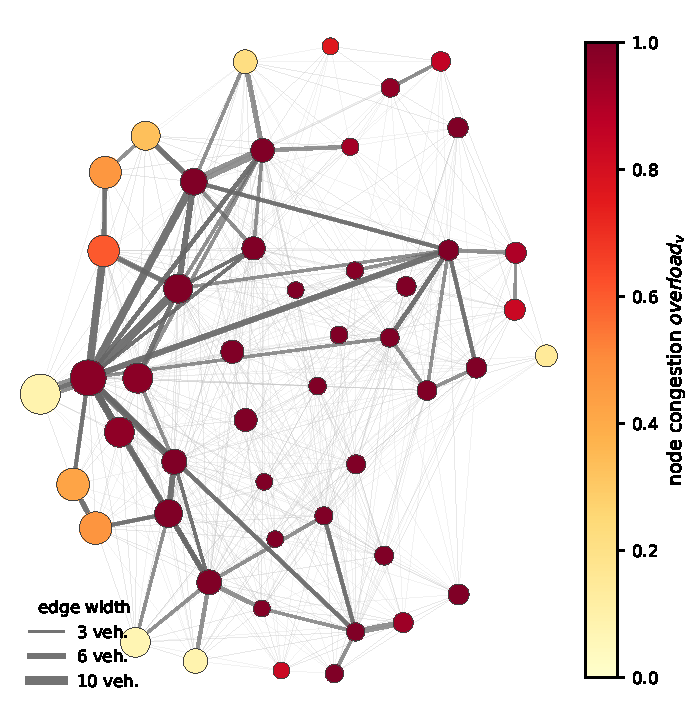
\includegraphics[width=0.37\textwidth]{figs/germany_solution.pdf}
\caption{A GVNS solution on the Germany real-geometry network ($|V|=49$), drawn
on its geographic layout. Node area encodes the transshipment capacity $W_v$ and
node colour the congestion $overload_v$ (dark $=$ at capacity). All used edges
are drawn faintly; backbone edges carrying at least three vehicles are emphasized
with width proportional to the vehicle count.}
\label{fig:solution}
\end{figure}

\subsection{Results}
Table~\ref{tab:results} summarises the synthetic and real-geometry results;
Figure~\ref{fig:ratios} plots the optimality gap and the reference ratios against
instance size. Four consistent trends emerge.

\emph{First, GVNS is near-optimal on small instances.} Its gap to the MIP dual
bound is only $0.96\%$ at $|V|=10$ and stays around $1$--$2\%$ up to
$|V|\approx20$, then grows with size ($4.8\%$ at $|V|=30$, $7.4\%$ at $|V|=50$),
reflecting the rapidly expanding path space. Since the dual bound is a valid lower bound, this
gap bounds the true distance of GVNS from the optimum rather than comparing it
against itself.

\emph{Second, the across-seed spread is small but grows with instance size, and
ten seeds are needed to see it.} On the synthetic instances the standard deviation
of the objective stays below $0.7\%$ of the mean at every size and below $0.2\%$ up
to $|V|=20$. On the largest real networks it is appreciably higher---$2.0\%$ on
Germany, $2.5\%$ on Italy, $2.2\%$ on European Russia---and, notably, three seeds
badly understate it: on Italy the spread measured over three seeds is $0.4\%$
against $2.5\%$ over ten. A single run is therefore representative on small
networks, whereas on capacity-tight instances the best of several runs is worth
taking.

\emph{Third, GVNS matches or beats the exact solver at equal time, increasingly
so with size.} On small instances the time-limited MIP incumbent essentially
ties GVNS ($Ratio_{\text{MIP}}\approx1.00$ for $|V|\le30$); from $|V|=45$ the
exact solver falls behind sharply, returning solutions $1.26$--$1.55\times$ more
expensive than GVNS at $|V|=49$--$59$. In other words, for a comparable
wall-clock budget the exact solver is up to $\sim\!55\%$ worse than GVNS. Tight
dual bounds are available up to $|V|=59$; for $|V|\gtrsim90$ the arc model reaches
millions of variables and the exact branch-and-bound becomes intractable, leaving
only the closed-form but loose LP-relaxation bound. Even there GVNS keeps
improving on its rounded-LP start by large factors ($2.2$--$3.0\times$,
Table~\ref{tab:results}).

\emph{Fourth, the real-geometry networks mirror the synthetic ones}: the gap to
the dual bound rises from $0.5\%$ (Denmark, $|V|=11$) to $11$--$16\%$ (Germany
$|V|=49$, Spain $|V|=59$), and the exact incumbent degrades from parity to
$1.3$--$1.5\times$ GVNS over the same range, corroborating both the fidelity of
the generator and the robustness of GVNS.

\begin{figure}[t]
\centering
\begin{subfigure}{0.47\textwidth}
  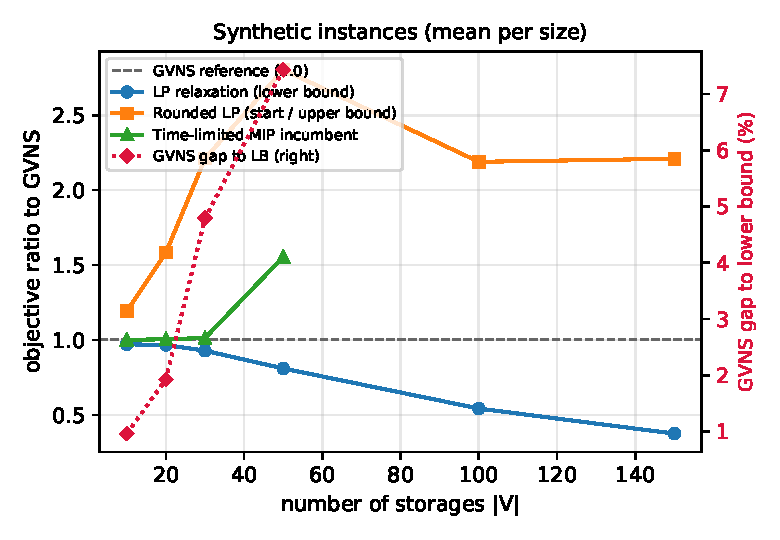
\includegraphics[width=\linewidth]{figs/synthetic_ratios.pdf}
  \caption{Synthetic instances (mean per size).}
  \label{fig:synth}
\end{subfigure}\hfill
\begin{subfigure}{0.47\textwidth}
  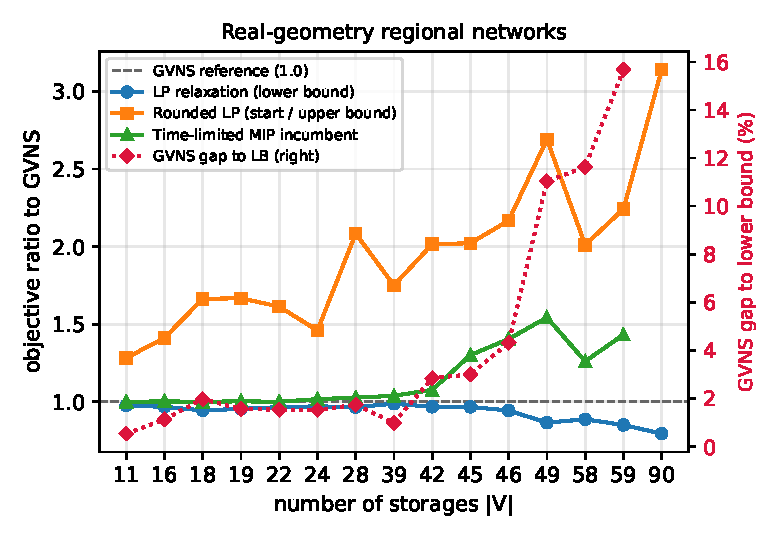
\includegraphics[width=\linewidth]{figs/real_ratios.pdf}
  \caption{Real-geometry regional networks.}
  \label{fig:real}
\end{subfigure}
\caption{Left axis: objective ratio of each reference method to GVNS versus network
size (below the line at $1.0$ is better than GVNS, above is worse). Right axis
(dotted): the GVNS gap to the best valid lower bound.}
\label{fig:ratios}
\end{figure}

% ---------------------------------------------------------------------
\begin{table}[t]
\centering
\caption{Results on the synthetic instances (top, aggregated by network size,
$n$ instances each) and on the real-geometry networks (bottom, one instance each).
$gap_{\mathrm{LB}}$ is the GVNS optimality gap to the best MIP dual bound, a valid
lower bound; the three middle columns are objective ratios of the LP relaxation,
the rounded LP and the time-limited MIP incumbent to GVNS; $\sigma$ is the
across-seed standard deviation as a fraction of the mean, $\bar t$ the mean GVNS
run time. ``$\dagger$'' marks sizes at which the arc model has millions of
variables and the exact branch-and-bound is intractable; the LP-relaxation and
rounded-LP bounds remain available in closed form.}
\label{tab:results}
\small
\setlength{\tabcolsep}{4pt}
\begin{tabular}{lccccccr}
\toprule
Instances & $|V|$ & $n$ & $gap_{\mathrm{LB}}$ & LP-relax. & Rounded LP
 & MIP-inc. & $\sigma$\\
\midrule
\multicolumn{8}{l}{\emph{Synthetic (mean per size)}}\\
& 10  & 10 & 0.96\% & 0.971 & 1.192 & 1.000 & 0.06\%\\
& 20  & 7  & 1.92\% & 0.966 & 1.583 & 1.005 & 0.18\%\\
& 30  & 7  & 4.79\% & 0.928 & 2.210 & 1.013 & 0.68\%\\
& 50  & 5  & 7.44\% & 0.810 & 2.804 & 1.555 & 0.66\%\\
& 100 & 3  & \dag & 0.542 & 2.189 & \dag & 0.31\%\\
& 150 & 3  & \dag & 0.375 & 2.210 & \dag & 0.38\%\\
\midrule
\multicolumn{8}{l}{\emph{Real-geometry regional networks}\hfill $\bar t$ (s)}\\
Denmark        & 11 & 1 & 0.5\%  & 0.977 & 1.283 & 1.000 & 615\\
Belgium        & 16 & 1 & 1.1\%  & 0.968 & 1.411 & 1.003 & 1292\\
Netherlands    & 18 & 1 & 2.0\%  & 0.945 & 1.664 & 1.000 & 1943\\
Hungary        & 19 & 1 & 1.6\%  & 0.955 & 1.668 & 1.003 & 1441\\
Ohio USA       & 22 & 1 & 1.5\%  & 0.965 & 1.614 & 1.000 & 1429\\
Georgia USA    & 24 & 1 & 1.5\%  & 0.971 & 1.460 & 1.017 & 2147\\
Illinois USA   & 28 & 1 & 1.7\%  & 0.966 & 2.085 & 1.027 & 2434\\
California USA & 39 & 1 & 1.0\%  & 0.988 & 1.751 & 1.039 & 2706\\
United Kingdom & 42 & 1 & 2.8\%  & 0.968 & 2.016 & 1.077 & 3343\\
Sweden         & 45 & 1 & 3.0\%  & 0.967 & 2.022 & 1.301 & 2812\\
Italy          & 46 & 1 & 4.3\%  & 0.944 & 2.169 & 1.405 & 2837\\
Germany        & 49 & 1 & 11.0\% & 0.866 & 2.692 & 1.544 & 3348\\
Texas USA      & 58 & 1 & 11.6\% & 0.887 & 2.012 & 1.261 & 3456\\
Spain          & 59 & 1 & 15.7\% & 0.851 & 2.243 & 1.433 & 3986\\
Europe Russia  & 90 & 1 & \dag & 0.795 & 3.141 & \dag & 5595\\
\bottomrule
\end{tabular}
\end{table}


\subsection{Algorithmic components}
\label{sec:ablation}

\begin{table}[t]
\centering
\caption{Contribution of each algorithmic component: \emph{median} objective
increase (best of five seeds) relative to the full GVNS on the same instances,
seeds and budget, over a representative subset of synthetic ($|V|=20$--$100$) and
real-geometry ($|V|=16$--$49$) instances. Medians are used because the across-seed
spread is heavy-tailed on the capacity-tight networks; means and maxima are quoted
in the text. $\bar t/\bar t_{\mathrm{GVNS}}$ is the run time relative to GVNS.}
\label{tab:components}
\small
\begin{tabular}{lccc}
\toprule
Variant & Synthetic & Real & $\bar t/\bar t_{\mathrm{GVNS}}$\\
\midrule
\multicolumn{4}{l}{\emph{Leave-one-out neighborhood ablation}}\\
without $N_1$ (reload-aware shortest paths) & $+0.8\%$ & $+0.8\%$ & $0.80$\\
without $N_2$ (partially loaded edges)      & $+4.0\%$ & $+1.6\%$ & $0.52$\\
without $N_3$ (congestion detours)          & $+0.1\%$ & $+0.2\%$ & $0.68$\\
\midrule
\multicolumn{4}{l}{\emph{Simplified search scheme}}\\
Basic VNS (local search restricted to $N_1$) & $+0.3\%$ & $+0.2\%$ & $0.63$\\
\bottomrule
\end{tabular}
\end{table}
Each component was assessed by re-running GVNS with it switched off, over five
seeds and the same budget, against the full method (Table~\ref{tab:components}).
$N_2$ (vehicle consolidation over partially loaded edges) is the dominant
operator: removing it costs $7.1\%$ on average and up to $23.8\%$ on the larger
synthetic instances, and $7.6\%$ on Germany, so filling spare vehicle capacity is
the main lever on the objective. $N_1$ contributes a smaller but consistent
improvement. $N_3$ (detours around congested storages) is \emph{situational}: it
is inactive when storages are far from their limit, but becomes valuable exactly
when the transshipment capacity binds---on Germany, where almost every storage
operates at capacity (Figure~\ref{fig:solution}), disabling it costs $4.0\%$.

The last row replaces the VND by a single-neighborhood local search over $N_1$,
keeping the same shake over $N_1$--$N_3$: this is the basic (``pure'') VNS, and
the gap to it measures what the \emph{general} part of GVNS is worth. That effect
is real but modest and strongly size-dependent. Counting an instance as decided
only when the difference exceeds the across-seed spread of both runs, GVNS wins
five of sixteen instances, Basic VNS one, and ten are ties; all but one decided
instance has $|V|\ge50$, where GVNS leads by $1.1$--$2.0\%$, whereas below
$|V|=30$ the two are indistinguishable. Basic VNS needs only $0.63$ of the GVNS
time, so it is preferable under a tight budget on small networks, while the full
VND earns its cost as the path space grows. The components are thus not equally
important: $N_2$ dominates, the VND structure matters mainly at scale, and $N_3$
is reserved for capacity-tight instances.



\section{Conclusion}
\label{sec:concl}
We addressed the design of logistic transport flows with nonlinear,
vehicle-induced edge costs and hard storage transshipment capacities, gave
arc-based and path-based MILP models with their relaxation, and proposed a GVNS
operating in the path space through three problem-specific neighborhoods.


On $35$ synthetic and $15$ real-geometry instances of up to $150$ storages, GVNS
came within about one percent of the best dual bound on small networks and, for a
comparable budget, was up to $55\%$ cheaper than a time-limited exact solver on
the medium ones; its optimality gap grows with size, as the path space explodes.
The component study showed that consolidating flow over partially loaded edges
($N_2$) is the dominant operator, that congestion detours ($N_3$) pay off only on
capacity-tight instances, and that the full VND is worth $1$--$2\%$ over a basic
VNS on the larger networks but nothing below $|V|=30$.

Two extensions stand out. The model treats capacities as static, whereas on real
networks both road throughput and reload demand vary with the time of day; moving
to a time-expanded graph with period-dependent $C_e(t)$ and $W_v(t)$, in the
spirit of time-dependent routing~\cite{gendreau2015tdr}, is a natural next step,
and the path-based GVNS carries over directly since its neighborhoods need only a
period-aware edge metric. Column-generation pricing could also feed the path pool
in place of the precomputed shortest-path pools, and validation on operational
data remains the ultimate test.

\subsubsection*{Code and data availability.}
The implementation, the exact-solver harness and the scripts that regenerate every
table and figure of Section~\ref{sec:experiments} are at
\url{https://github.com/aponom84/Optimal-Logistic-Net}; the instances are on
Zenodo~\cite{benchmark-data} under CC-BY-4.0.

\subsubsection*{Acknowledgements.}
The study was implemented in the framework of the Basic Research Program at
HSE University (HSE-BR-2025-080).
Also, this research was supported in part through computational resources of HPC facilities at HSE University.


\FloatBarrier
\begin{thebibliography}{99}
\small
\bibitem{alumur2008} Alumur, S., Kara, B.Y.: Network hub location problems: the
state of the art. Eur. J. Oper. Res. \textbf{190}(1), 1--21 (2008)
\bibitem{amous2017} Amous, M., Toumi, S., Jarboui, B., Eddaly, M.: A variable
neighborhood search algorithm for the capacitated vehicle routing problem.
Comput. Oper. Res. \textbf{88}, 234--248 (2017)
\bibitem{barnhart1998} Barnhart, C., Johnson, E.L., Nemhauser, G.L.,
Savelsbergh, M.W.P., Vance, P.H.: Branch-and-price: column generation for
solving huge integer programs. Oper. Res. \textbf{46}(3), 316--329 (1998)
\bibitem{barthelemy2011} Barth\'elemy, M.: Spatial networks. Phys. Rep.
\textbf{499}(1--3), 1--101 (2011)
\bibitem{batsyn2014ttrp} Batsyn, M., Ponomarenko, A.: Heuristic for a real-life
truck and trailer routing problem. Procedia Comput. Sci. \textbf{31}, 778--792
(2014)
\bibitem{batsyn2015heuristic} Batsyn, M., Ponomarenko, A.: Heuristic for
site-dependent truck and trailer routing problem with soft and hard time windows
and split deliveries. In: Pardalos, P., Pavone, M., Farinella, G.M., Cutello, V.
(eds.) MOD 2015. LNCS, vol.~9432, pp.~65--79. Springer, Cham (2015)
\bibitem{crainic2000} Crainic, T.G.: Service network design in freight
transportation. Eur. J. Oper. Res. \textbf{122}(2), 272--288 (2000)
\bibitem{crainic2021} Crainic, T.G., Gendreau, M.: Heuristics and metaheuristics
for fixed-charge network design. In: Crainic, T.G., Gendron, B., Gendreau, M.
(eds.) Network Design with Applications to Transportation and Logistics,
pp.~91--138. Springer, Cham (2021)
\bibitem{croxton2003} Croxton, K.L., Gendron, B., Magnanti, T.L.: A comparison
of mixed-integer programming models for nonconvex piecewise linear cost
minimization problems. Manage. Sci. \textbf{49}(9), 1268--1273 (2003)
\bibitem{gabaix1999} Gabaix, X.: Zipf's law for cities: an explanation. Q. J.
Econ. \textbf{114}(3), 739--767 (1999)
\bibitem{gabrel1999} Gabrel, V., Knippel, A., Minoux, M.: Exact solution of
multicommodity network optimization problems with general step cost functions.
Oper. Res. Lett. \textbf{25}(1), 15--23 (1999)
\bibitem{gastner2006} Gastner, M.T., Newman, M.E.J.: The spatial structure of
networks. Eur. Phys. J. B \textbf{49}(2), 247--252 (2006)
\bibitem{gendreau2015tdr} Gendreau, M., Ghiani, G., Guerriero, E.:
Time-dependent routing problems: a review. Comput. Oper. Res. \textbf{64},
189--197 (2015)
\bibitem{gendron1999} Gendron, B., Crainic, T.G., Frangioni, A.: Multicommodity
capacitated network design. In: Sans\`o, B., Soriano, P. (eds.)
Telecommunications Network Planning, pp.~1--19. Kluwer, Boston (1999)
\bibitem{ghamlouche2003} Ghamlouche, I., Crainic, T.G., Gendreau, M.:
Cycle-based neighbourhoods for fixed-charge capacitated multicommodity network
design. Oper. Res. \textbf{51}(4), 655--667 (2003)
\bibitem{hansen2019} Hansen, P., Mladenovi\'c, N.: Variable neighborhood search.
In: Handbook of Metaheuristics, 3rd edn., pp.~57--97. Springer, Cham (2019)
\bibitem{hansen2017} Hansen, P., Mladenovi\'c, N., Todosijevi\'c, R., Hanafi, S.:
Variable neighborhood search: basics and variants. EURO J. Comput. Optim.
\textbf{5}(3), 423--454 (2017)
\bibitem{hewitt2010} Hewitt, M., Nemhauser, G.L., Savelsbergh, M.W.P.: Combining
exact and heuristic approaches for the capacitated fixed-charge network flow
problem. INFORMS J. Comput. \textbf{22}(2), 314--325 (2010)
\bibitem{scip} Hojny, C., Besan\c{c}on, M., Bestuzheva, K., et al.: The SCIP
Optimization Suite 10.0. arXiv:2511.18580 (2025)
\bibitem{highs} Huangfu, Q., Hall, J.A.J.: Parallelizing the dual revised simplex
method. Math. Program. Comput. \textbf{10}(1), 119--142 (2018)
\bibitem{karakostas2019} Karakostas, P., Sifaleras, A., Georgiadis, M.C.: A
general variable neighborhood search-based solution approach for the
location-inventory routing problem with distribution outsourcing. Comput. Chem.
Eng. \textbf{126}, 263--279 (2019)
\bibitem{kirkley2018} Kirkley, A., Barbosa, H., Barthelemy, M., Ghoshal, G.:
From networks to optimal higher-order models of complex systems. Nat. Phys.
\textbf{14}, 250--258 (2018)
\bibitem{charisma} Kostenetskiy, P., Kozyrev, V., Chulkevich, R., Salikova, M.,
Mishenin, R.: High-performance computing at HSE University. In: Sokolinsky, L.,
Zymbler, M., Voevodin, V., Dongarra, J. (eds.) Parallel Computational
Technologies, pp.~17--29. Springer, Cham (2026)
\bibitem{benchmark} Kovaleva, V., Ponomarenko, A.: A benchmark generator of
realistic logistic transport networks with nonlinear edge costs and
transshipment capacities. arXiv:2606.20653 (2026)
\bibitem{benchmark-data} Kovaleva, V., Ponomarenko, A.: A benchmark of realistic
logistic transport networks with nonlinear edge costs and transshipment
capacities (dataset). Zenodo (2026).
\url{https://doi.org/10.5281/zenodo.20372456}
\bibitem{masri2015} Masri, H., Krichen, S., Guitouni, A.: A multi-start variable
neighborhood search for solving the single path multicommodity flow problem.
Appl. Math. Comput. \textbf{251}, 132--142 (2015)
\bibitem{mjirda2014} Mjirda, A., Jarboui, B., Mladenovi\'c, J., Wilbaut, C.,
Hanafi, S.: A general variable neighbourhood search for the multi-product
inventory routing problem. IMA J. Manag. Math. \textbf{27}(1) (2016)
\bibitem{mladenovic1997} Mladenovi\'c, N., Hansen, P.: Variable neighborhood
search. Comput. Oper. Res. \textbf{24}(11), 1097--1100 (1997)
\bibitem{osm} OpenStreetMap. \url{https://www.openstreetmap.org} (accessed
2026-04-11)
\bibitem{rodriguez2010} Rodr\'iguez-Mart\'in, I., Salazar-Gonz\'alez, J.J.: A
local branching heuristic for the capacitated fixed-charge network design
problem. Comput. Oper. Res. \textbf{37}(3), 575--581 (2010)
\bibitem{wilson1967} Wilson, A.G.: A statistical theory of spatial distribution
models. Transp. Res. \textbf{1}(3), 253--269 (1967)
\end{thebibliography}

\end{document}
